\chapter{Digital representation of music}\label{ch:digital-audio-representation}

\begin{chapterabstract}
    In reality, sounds manifest as continuous \textit{waves} propagating through a medium (like air).
    On the other hand, personal computers are \textit{digital} by design and cannot \textit{easily} represent \textit{continuous} information;
    therefore, when storing audio in a computer, we have to perform conversions for the computer to accommodate our audio track.
    This chapter will look over possible representations of music representation in a computer.
\end{chapterabstract}


\section{Wave representation}\label{sec:wave-representation}

The first possible option when representing an audio track in a computer is to try and capture characteristics of the beforementioned \textit{sound wave}.
In order to manipulate this \textit{continuous signal} via a digital computer, the signal must be digitalized with an \textit{analog-to-digital converter} (A/D).
The converter repeatedly samples the instantaneous \textit{voltage amplitude} of the \textit{analog} input signal at a given sample rate, commonly thousands or tens of thousands of times per second.
In the audio signal, the measured voltage of the input signal is proportional to the sound pressure measured by a device such as a \textit{microphone}.
The final discrete representation of the converted signal created by the converter consists of a sequence of numeric values (hence the term digital) representing the amplitude of the original waveform at evenly spaced points in time.~\cite{sound-representation}

\begin{figure}
    \centering
    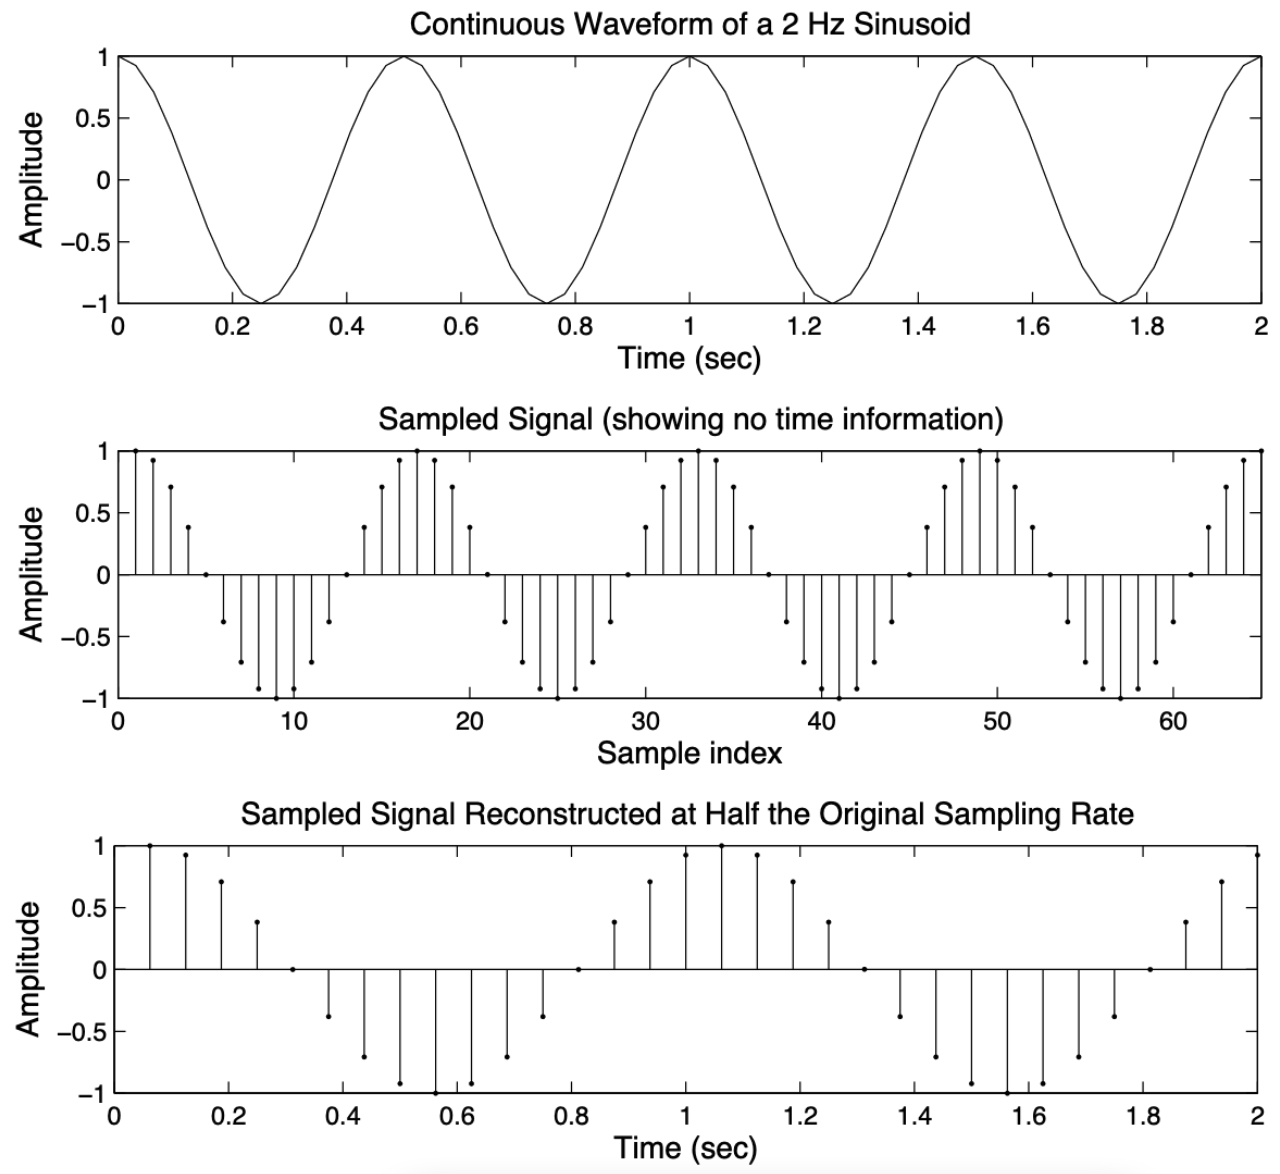
\includegraphics[width=0.7\textwidth]{assets/sound-sampling}
    \caption{~Digitization of signal via sampling~\cite{smyth_2019}}\label{fig:sound-digitization}
\end{figure}


\section{Symbolic representation}\label{sec:symbolic-representation}

Another option is to represent music \textit{symbolically}.
Unlike the wave representation, which represents music (any audio generally) in a low-level physical fashion, the symbolic representation uses \textit{special symbols} to represent different musical elements like notes and rests.

The downside of this representation is that it can only depict specific musical instruments, unlike wave representation, which can also depict vocals and arbitrary sounds.
However, this approach is much better suited for our application, as it expresses the essential musical properties.
Therefore, it will be much easier for our neural nets to learn the intrinsic properties of compositions provided as learning data and thus will presumably be more successful at imitating them.
We will now go over the most common symbolic formats for music.

\subsection{MIDI}\label{subsec:midi}

The MIDI abbreviation stands for the \textit{Musical Instrument Digital Interface}.
It is a protocol developed in the early 1980s to standardize the \textit{exchange and storage} of musical information.
It is the most widespread \textit{binary} communication protocol intended to connect electronic musical instruments such as synthesizers and other electronic music equipment to a computer for recording, editing, and programming.
MIDI protocol appeared as a response to the need to standardize the communication between the synthesizers and other musical equipment and was created when electronic music was developed by a consortium of Japanese and American manufacturers of Synthesizers (Sequential Systems, Roland Corporation, Yamaha, Kurzweil, \ldots).
It is used to transmit data using serial ports but can also be written to a file and be used as a means of storage.
MIDI is an extensive standard consisting of hardware, drivers, communication channels, messages, modes, controllers, visual effects control, and a file format standard.
In this work, we will only concern ourselves with the \textit{MIDI file format}, as it is the thing that we will need during the implementation part.
Since the protocol was developed in the 80s, it was designed to have low overhead and, therefore, \textit{low-level}.
We do not need to go into the detail of binary encoding used to describe different MIDI events;
instead, we will present an abstracted high-level overview, which is sufficient for our application.~\cite{understanding-midi}

\subsubsection{MIDI file format}\label{subsubsec:midi-file-format}

The MIDI file starts with a header, where the format type (single track, multiple synchronous tracks, or multiple asynchronous tracks), the number of tracks, and time division (ticks per beat).
The file body composes of an array of MIDI \textit{messages}.
Each message denotes the message content and $\Delta$ (delta) time;
the amount of ticks the event is shifted after the preceding event.
There are some \textit{meta-messages} that specify additional information like song lyrics, tempo, state end of the track, and others.
There are multiple message types like \texttt{control\_change} for specifying pedal/slider position or program change to choose one of 128 instruments.
However, the most substantial messages are \texttt{note\_on} and \texttt{note\_off}.
These take arguments pitch (0-127) and velocity (0-127) and specify the pressing and releasing of a note specified by pitch number.
The velocity controls the force of a note being pressed.
Zero velocity has the same meaning as the \texttt{note\_off} message, so the release of a key.
Please take a look at figure~\ref{fig:score-to-midi}, which contains an example of a score.~\cite{understanding-midi}

\begin{figure}
    \centering
    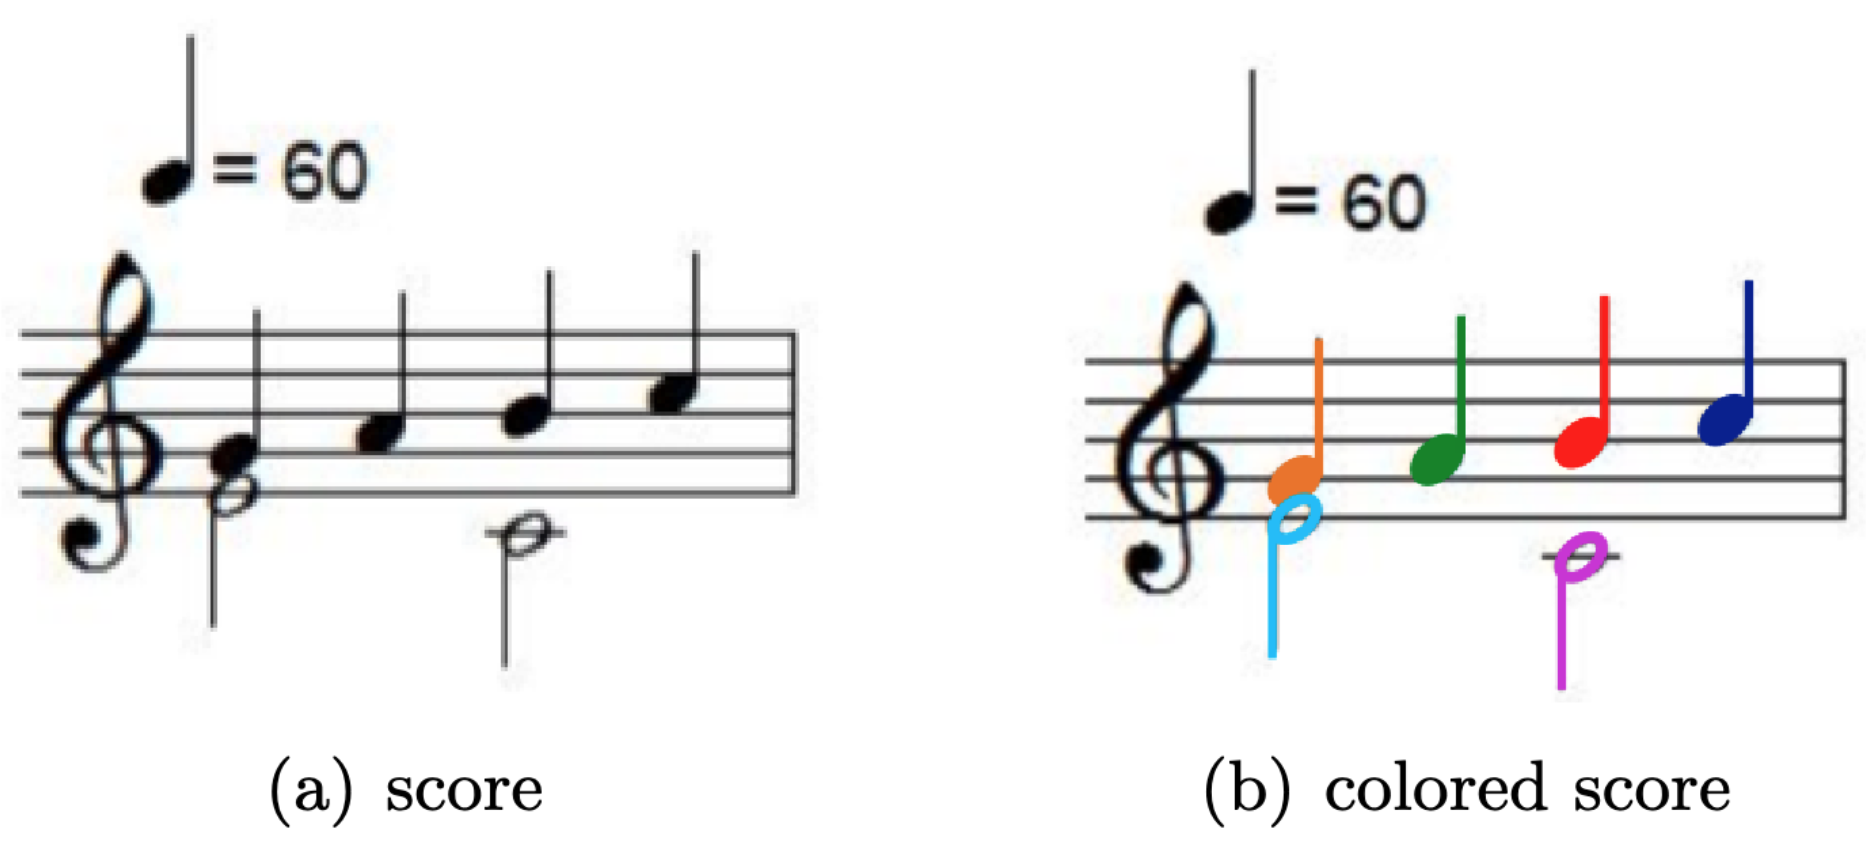
\includegraphics[width=0.4\textwidth]{assets/score-to-midi}
    \caption{~Example of a musical score~\cite{understanding-midi}}\label{fig:score-to-midi}
\end{figure}

This would translate into following messages in MIDI:

\begin{center}
    \begin{tabular}{ |c|c|c| }
        \hline
        \textbf{midi message} & \textbf{pitch} & \textbf{note value}    \\
        \hline
        \texttt{note\_on}     & 64             & \textcolor{cyan}{E4}   \\
        \texttt{note\_on}     & 67             & \textcolor{orange}{G4} \\
        \texttt{note\_off}    & 67             & \textcolor{orange}{G4} \\
        \texttt{note\_on}     & 69             & \textcolor{Green}{A4}  \\
        \texttt{note\_off}    & 69             & \textcolor{Green}{A4}  \\
        \texttt{note\_off}    & 64             & \textcolor{cyan}{E4}   \\
        \texttt{note\_on}     & 60             & \textcolor{violet}{C4} \\
        \texttt{note\_on}     & 71             & \textcolor{red}{B4}    \\
        \texttt{note\_off}    & 71             & \textcolor{red}{B4}    \\
        \texttt{note\_on}     & 72             & \textcolor{blue}{C5}   \\
        \texttt{note\_off}    & 72             & \textcolor{blue}{C5}   \\
        \texttt{note\_off}    & 60             & \textcolor{violet}{C4} \\
        \hline
    \end{tabular}
\end{center}
